\documentclass{article}
\usepackage{tikz}
\usetikzlibrary{shapes, arrows.meta, positioning, backgrounds}

\begin{document}

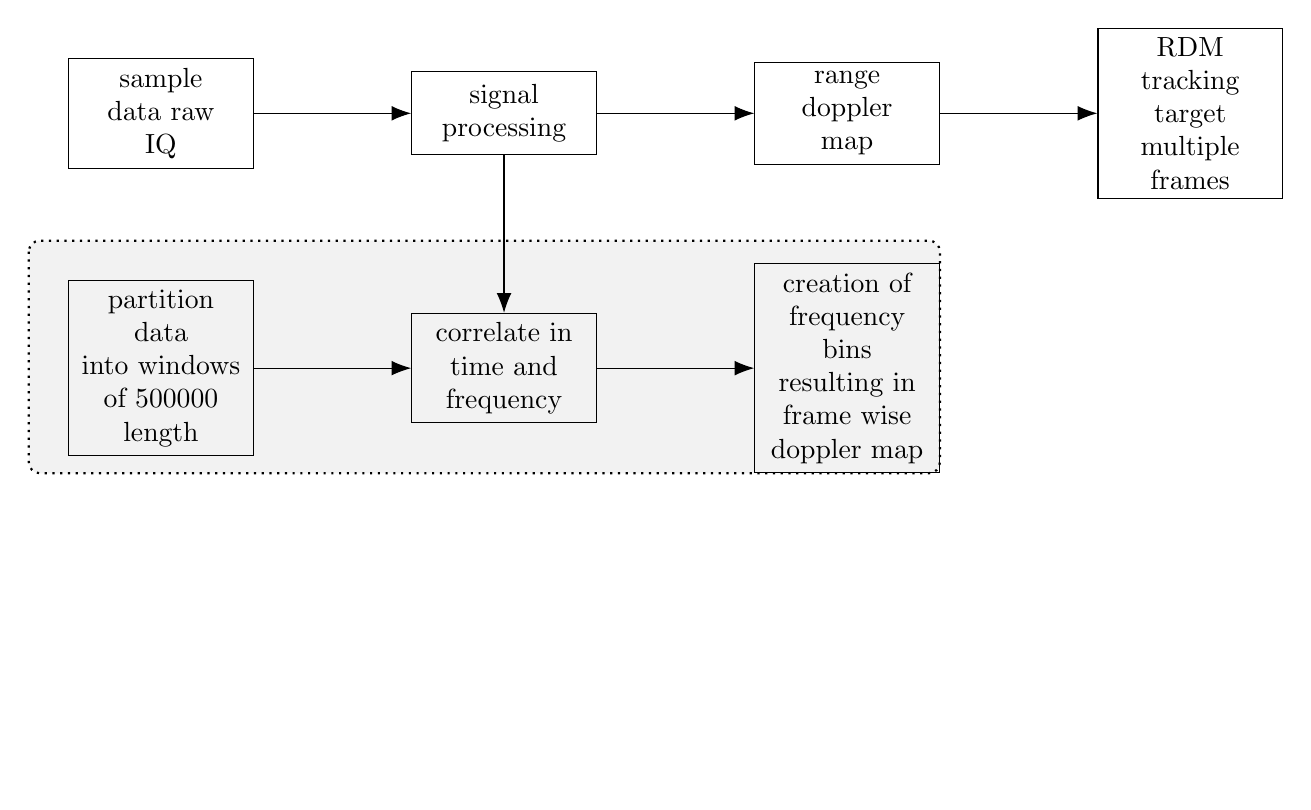
\begin{tikzpicture}[auto, node distance=2cm, >=Latex]
    % Define the styles
    \tikzset{
        block/.style = {draw, rectangle, minimum height=3em, text width=6em, align=center}, % Adjusted text width
        line/.style = {draw, -{Latex[length=2.5mm]}},
    }

    % Nodes placement
    \node [block] (sample) {sample data raw \\ IQ};
    \node [block, right=of sample] (processing) {signal \\ processing};
    \node [block, right=of processing] (map) {range \\ doppler \\ map};
    \node [block, right=of map] (track) {RDM \\ tracking target \\ multiple frames};

    % Subblocks
    \node [block, below=of processing] (sub2) {correlate in \\ time and \\ frequency};
    \node [block, left=of sub2] (sub1) {partition data \\ into windows \\ of 500000 \\ length};
    \node [block, right=of sub2] (sub3) {creation of \\ frequency bins \\ resulting in \\ frame wise \\ doppler map};

    % Draw rectangle around subblocks
    \begin{pgfonlayer}{background}
        \draw[draw=black, fill=gray!10, dotted, rounded corners, thick] (sub1.west |- sub1.north) ++(-0.5,0.5) rectangle (sub3.east |- sub3.south) ++(3.4,-3.9);
    \end{pgfonlayer}


    % Connecting lines
    \draw [line] (sample) -- (processing);
    \draw [line] (processing) -- (map);
    \draw [line] (sub1) -- (sub2);
    \draw [line] (sub2) -- (sub3);
    \draw [line] (processing) -- (sub2);
    \draw [line] (map) -- (track);

    % Additional decorative lines (dotted lines to indicate grouping or flow)
    \draw [dotted] (processing.south) -- (sub2.north);

\end{tikzpicture}


\end{document}
